\documentclass[twoside]{book}

% Packages required by doxygen
\usepackage{fixltx2e}
\usepackage{calc}
\usepackage{doxygen}
\usepackage[export]{adjustbox} % also loads graphicx
\usepackage{graphicx}
\usepackage[utf8]{inputenc}
\usepackage{makeidx}
\usepackage{multicol}
\usepackage{multirow}
\PassOptionsToPackage{warn}{textcomp}
\usepackage{textcomp}
\usepackage[nointegrals]{wasysym}
\usepackage[table]{xcolor}

% Font selection
\usepackage[T1]{fontenc}
\usepackage[scaled=.90]{helvet}
\usepackage{courier}
\usepackage{amssymb}
\usepackage{sectsty}
\renewcommand{\familydefault}{\sfdefault}
\allsectionsfont{%
  \fontseries{bc}\selectfont%
  \color{darkgray}%
}
\renewcommand{\DoxyLabelFont}{%
  \fontseries{bc}\selectfont%
  \color{darkgray}%
}
\newcommand{\+}{\discretionary{\mbox{\scriptsize$\hookleftarrow$}}{}{}}

% Page & text layout
\usepackage{geometry}
\geometry{%
  a4paper,%
  top=2.5cm,%
  bottom=2.5cm,%
  left=2.5cm,%
  right=2.5cm%
}
\tolerance=750
\hfuzz=15pt
\hbadness=750
\setlength{\emergencystretch}{15pt}
\setlength{\parindent}{0cm}
\setlength{\parskip}{3ex plus 2ex minus 2ex}
\makeatletter
\renewcommand{\paragraph}{%
  \@startsection{paragraph}{4}{0ex}{-1.0ex}{1.0ex}{%
    \normalfont\normalsize\bfseries\SS@parafont%
  }%
}
\renewcommand{\subparagraph}{%
  \@startsection{subparagraph}{5}{0ex}{-1.0ex}{1.0ex}{%
    \normalfont\normalsize\bfseries\SS@subparafont%
  }%
}
\makeatother

% Headers & footers
\usepackage{fancyhdr}
\pagestyle{fancyplain}
\fancyhead[LE]{\fancyplain{}{\bfseries\thepage}}
\fancyhead[CE]{\fancyplain{}{}}
\fancyhead[RE]{\fancyplain{}{\bfseries\leftmark}}
\fancyhead[LO]{\fancyplain{}{\bfseries\rightmark}}
\fancyhead[CO]{\fancyplain{}{}}
\fancyhead[RO]{\fancyplain{}{\bfseries\thepage}}
\fancyfoot[LE]{\fancyplain{}{}}
\fancyfoot[CE]{\fancyplain{}{}}
\fancyfoot[RE]{\fancyplain{}{\bfseries\scriptsize Generated by Doxygen }}
\fancyfoot[LO]{\fancyplain{}{\bfseries\scriptsize Generated by Doxygen }}
\fancyfoot[CO]{\fancyplain{}{}}
\fancyfoot[RO]{\fancyplain{}{}}
\renewcommand{\footrulewidth}{0.4pt}
\renewcommand{\chaptermark}[1]{%
  \markboth{#1}{}%
}
\renewcommand{\sectionmark}[1]{%
  \markright{\thesection\ #1}%
}

% Indices & bibliography
\usepackage{natbib}
\usepackage[titles]{tocloft}
\setcounter{tocdepth}{3}
\setcounter{secnumdepth}{5}
\makeindex

% Hyperlinks (required, but should be loaded last)
\usepackage{ifpdf}
\ifpdf
  \usepackage[pdftex,pagebackref=true]{hyperref}
\else
  \usepackage[ps2pdf,pagebackref=true]{hyperref}
\fi
\hypersetup{%
  colorlinks=true,%
  linkcolor=blue,%
  citecolor=blue,%
  unicode%
}

% Custom commands
\newcommand{\clearemptydoublepage}{%
  \newpage{\pagestyle{empty}\cleardoublepage}%
}

\usepackage{caption}
\captionsetup{labelsep=space,justification=centering,font={bf},singlelinecheck=off,skip=4pt,position=top}

%===== C O N T E N T S =====

\begin{document}

% Titlepage & ToC
\hypersetup{pageanchor=false,
             bookmarksnumbered=true,
             pdfencoding=unicode
            }
\pagenumbering{roman}
\begin{titlepage}
\vspace*{7cm}
\begin{center}%
{\Large My Project }\\
\vspace*{1cm}
{\large Generated by Doxygen 1.8.11}\\
\end{center}
\end{titlepage}
\clearemptydoublepage
\tableofcontents
\clearemptydoublepage
\pagenumbering{arabic}
\hypersetup{pageanchor=true}

%--- Begin generated contents ---
\chapter{Class Index}
\section{Class List}
Here are the classes, structs, unions and interfaces with brief descriptions\+:\begin{DoxyCompactList}
\item\contentsline{section}{\hyperlink{structmarket__rates__struct}{market\+\_\+rates\+\_\+struct} \\*Estructura de memoria compartida de cotizaciones }{\pageref{structmarket__rates__struct}}{}
\item\contentsline{section}{\hyperlink{structmsgbuf}{msgbuf} \\*Estructura de colas de mensajes }{\pageref{structmsgbuf}}{}
\item\contentsline{section}{\hyperlink{structrace__control__struct}{race\+\_\+control\+\_\+struct} \\*Estructura de memoria compartida de control de carrera }{\pageref{structrace__control__struct}}{}
\end{DoxyCompactList}

\chapter{File Index}
\section{File List}
Here is a list of all documented files with brief descriptions\+:\begin{DoxyCompactList}
\item\contentsline{section}{\hyperlink{ejercicio2_8c}{ejercicio2.\+c} \\*Ejercicio2 Creación de 4 procesos hijos que duermen durante 30s mientras que el proceso padre espera 5s y después envía a cada proceso hijo la señal de finalización S\+I\+G\+T\+E\+RM }{\pageref{ejercicio2_8c}}{}
\item\contentsline{section}{\hyperlink{ejercicio4_8c}{ejercicio4.\+c} \\*Ejercicio4 Manejo de señales entre procesos hijos y padre }{\pageref{ejercicio4_8c}}{}
\item\contentsline{section}{\hyperlink{ejercicio6a_8c}{ejercicio6a.\+c} \\*Ejercicio6a Toma de contacto con la funcion alarm() }{\pageref{ejercicio6a_8c}}{}
\item\contentsline{section}{\hyperlink{ejercicio6b_8c}{ejercicio6b.\+c} \\*Ejercicio6b Toma de contacto con la funcion sigfillset() }{\pageref{ejercicio6b_8c}}{}
\item\contentsline{section}{\hyperlink{semaforos_8c}{semaforos.\+c} \\*Ejercicio9 }{\pageref{semaforos_8c}}{}
\item\contentsline{section}{\hyperlink{semaforos_8h}{semaforos.\+h} \\*Utilidades de manejo de semaforos }{\pageref{semaforos_8h}}{}
\end{DoxyCompactList}

\chapter{Class Documentation}
\hypertarget{structmarket__rates__struct}{}\section{market\+\_\+rates\+\_\+struct Struct Reference}
\label{structmarket__rates__struct}\index{market\+\_\+rates\+\_\+struct@{market\+\_\+rates\+\_\+struct}}


Estructura de memoria compartida de cotizaciones.  


\subsection*{Public Attributes}
\begin{DoxyCompactItemize}
\item 
float \hyperlink{structmarket__rates__struct_a364e28430ed23ff65270f5124d94f932}{horse\+\_\+bet} \mbox{[}\hyperlink{proyecto_8c_a1f292d5e7fb89ea56519859a22db34c6}{M\+A\+X\+\_\+\+H\+O\+R\+S\+ES}\mbox{]}
\item 
float \hyperlink{structmarket__rates__struct_ad3c6f2f118a4c411a8035256851d141a}{horse\+\_\+rate} \mbox{[}\hyperlink{proyecto_8c_a1f292d5e7fb89ea56519859a22db34c6}{M\+A\+X\+\_\+\+H\+O\+R\+S\+ES}\mbox{]}
\item 
float \hyperlink{structmarket__rates__struct_afabd309263178532df483c3f56acb586}{total}
\end{DoxyCompactItemize}


\subsection{Detailed Description}
Estructura de memoria compartida de cotizaciones. 

Esta estructura contiene la informacion de las cotizaciones en la etapa de apuestas 

\subsection{Member Data Documentation}
\index{market\+\_\+rates\+\_\+struct@{market\+\_\+rates\+\_\+struct}!horse\+\_\+bet@{horse\+\_\+bet}}
\index{horse\+\_\+bet@{horse\+\_\+bet}!market\+\_\+rates\+\_\+struct@{market\+\_\+rates\+\_\+struct}}
\subsubsection[{\texorpdfstring{horse\+\_\+bet}{horse_bet}}]{\setlength{\rightskip}{0pt plus 5cm}float market\+\_\+rates\+\_\+struct\+::horse\+\_\+bet\mbox{[}{\bf M\+A\+X\+\_\+\+H\+O\+R\+S\+ES}\mbox{]}}\hypertarget{structmarket__rates__struct_a364e28430ed23ff65270f5124d94f932}{}\label{structmarket__rates__struct_a364e28430ed23ff65270f5124d94f932}
Apuestas totoles a cada caballo \index{market\+\_\+rates\+\_\+struct@{market\+\_\+rates\+\_\+struct}!horse\+\_\+rate@{horse\+\_\+rate}}
\index{horse\+\_\+rate@{horse\+\_\+rate}!market\+\_\+rates\+\_\+struct@{market\+\_\+rates\+\_\+struct}}
\subsubsection[{\texorpdfstring{horse\+\_\+rate}{horse_rate}}]{\setlength{\rightskip}{0pt plus 5cm}float market\+\_\+rates\+\_\+struct\+::horse\+\_\+rate\mbox{[}{\bf M\+A\+X\+\_\+\+H\+O\+R\+S\+ES}\mbox{]}}\hypertarget{structmarket__rates__struct_ad3c6f2f118a4c411a8035256851d141a}{}\label{structmarket__rates__struct_ad3c6f2f118a4c411a8035256851d141a}
Cotizacion de cada caballo \index{market\+\_\+rates\+\_\+struct@{market\+\_\+rates\+\_\+struct}!total@{total}}
\index{total@{total}!market\+\_\+rates\+\_\+struct@{market\+\_\+rates\+\_\+struct}}
\subsubsection[{\texorpdfstring{total}{total}}]{\setlength{\rightskip}{0pt plus 5cm}float market\+\_\+rates\+\_\+struct\+::total}\hypertarget{structmarket__rates__struct_afabd309263178532df483c3f56acb586}{}\label{structmarket__rates__struct_afabd309263178532df483c3f56acb586}
Cantidad total apostada 

The documentation for this struct was generated from the following file\+:\begin{DoxyCompactItemize}
\item 
\hyperlink{proyecto_8c}{proyecto.\+c}\end{DoxyCompactItemize}

\hypertarget{structmsgbuf}{}\section{msgbuf Struct Reference}
\label{structmsgbuf}\index{msgbuf@{msgbuf}}


Estructura de colas de mensajes.  


\subsection*{Public Attributes}
\begin{DoxyCompactItemize}
\item 
long \hyperlink{structmsgbuf_a12a4780abaa96553f2ebf5fafeb58360}{mtype}
\item 
\begin{tabbing}
xx\=xx\=xx\=xx\=xx\=xx\=xx\=xx\=xx\=\kill
struct \{\\
\>struct \{\\
\>\>char \hyperlink{structmsgbuf_a72921f6ad2d6985d78d0e0fd1ae00774}{name} \mbox{[}\hyperlink{proyecto_8c_a834e9a379307f869a10f4da078be5786}{NAME\_SIZE}\mbox{]}\\
\>\>int \hyperlink{structmsgbuf_a4d6daa3e4bf410b275b596b1e6828110}{bettor\_id}\\
\>\>int \hyperlink{structmsgbuf_a2d569f43a4859884c21c9ce8f1408eeb}{horse\_id}\\
\>\>float \hyperlink{structmsgbuf_a39278db78542cbe8cf2df77ac5b8b080}{bet}\\
\>\} \hyperlink{structmsgbuf_a1337d4cd36a0fa762c15244c00853381}{betting}\\
\>struct \{\\
\>\>int \hyperlink{structmsgbuf_a0a654069b1868c3be58115550ed078fa}{position}\\
\>\>int \hyperlink{structmsgbuf_a2b1acedae627a698a89d2503665c593d}{last\_throw}\\
\>\} {\bfseries race}\\
\} \hyperlink{structmsgbuf_ad43d12674488c373d8fb69efed53c3cc}{info}\\

\end{tabbing}\end{DoxyCompactItemize}


\subsection{Detailed Description}
Estructura de colas de mensajes. 

Esta estructura contiene la informacion necesaria para comunicarse por colas de mensajes 

\subsection{Member Data Documentation}
\index{msgbuf@{msgbuf}!bet@{bet}}
\index{bet@{bet}!msgbuf@{msgbuf}}
\subsubsection[{\texorpdfstring{bet}{bet}}]{\setlength{\rightskip}{0pt plus 5cm}float msgbuf\+::bet}\hypertarget{structmsgbuf_a39278db78542cbe8cf2df77ac5b8b080}{}\label{structmsgbuf_a39278db78542cbe8cf2df77ac5b8b080}
cantidad apostada \index{msgbuf@{msgbuf}!betting@{betting}}
\index{betting@{betting}!msgbuf@{msgbuf}}
\subsubsection[{\texorpdfstring{betting}{betting}}]{\setlength{\rightskip}{0pt plus 5cm}struct \{ ... \}  msgbuf\+::betting}\hypertarget{structmsgbuf_a1337d4cd36a0fa762c15244c00853381}{}\label{structmsgbuf_a1337d4cd36a0fa762c15244c00853381}
Informacion de apuestas \index{msgbuf@{msgbuf}!bettor\+\_\+id@{bettor\+\_\+id}}
\index{bettor\+\_\+id@{bettor\+\_\+id}!msgbuf@{msgbuf}}
\subsubsection[{\texorpdfstring{bettor\+\_\+id}{bettor_id}}]{\setlength{\rightskip}{0pt plus 5cm}int msgbuf\+::bettor\+\_\+id}\hypertarget{structmsgbuf_a4d6daa3e4bf410b275b596b1e6828110}{}\label{structmsgbuf_a4d6daa3e4bf410b275b596b1e6828110}
ID apostador \index{msgbuf@{msgbuf}!horse\+\_\+id@{horse\+\_\+id}}
\index{horse\+\_\+id@{horse\+\_\+id}!msgbuf@{msgbuf}}
\subsubsection[{\texorpdfstring{horse\+\_\+id}{horse_id}}]{\setlength{\rightskip}{0pt plus 5cm}int msgbuf\+::horse\+\_\+id}\hypertarget{structmsgbuf_a2d569f43a4859884c21c9ce8f1408eeb}{}\label{structmsgbuf_a2d569f43a4859884c21c9ce8f1408eeb}
ID caballo \index{msgbuf@{msgbuf}!info@{info}}
\index{info@{info}!msgbuf@{msgbuf}}
\subsubsection[{\texorpdfstring{info}{info}}]{\setlength{\rightskip}{0pt plus 5cm}struct \{ ... \}  msgbuf\+::info}\hypertarget{structmsgbuf_ad43d12674488c373d8fb69efed53c3cc}{}\label{structmsgbuf_ad43d12674488c373d8fb69efed53c3cc}
Informacion de control de carrera \index{msgbuf@{msgbuf}!last\+\_\+throw@{last\+\_\+throw}}
\index{last\+\_\+throw@{last\+\_\+throw}!msgbuf@{msgbuf}}
\subsubsection[{\texorpdfstring{last\+\_\+throw}{last_throw}}]{\setlength{\rightskip}{0pt plus 5cm}int msgbuf\+::last\+\_\+throw}\hypertarget{structmsgbuf_a2b1acedae627a698a89d2503665c593d}{}\label{structmsgbuf_a2b1acedae627a698a89d2503665c593d}
ultima tirada \index{msgbuf@{msgbuf}!mtype@{mtype}}
\index{mtype@{mtype}!msgbuf@{msgbuf}}
\subsubsection[{\texorpdfstring{mtype}{mtype}}]{\setlength{\rightskip}{0pt plus 5cm}long msgbuf\+::mtype}\hypertarget{structmsgbuf_a12a4780abaa96553f2ebf5fafeb58360}{}\label{structmsgbuf_a12a4780abaa96553f2ebf5fafeb58360}
tipo del mensaje \index{msgbuf@{msgbuf}!name@{name}}
\index{name@{name}!msgbuf@{msgbuf}}
\subsubsection[{\texorpdfstring{name}{name}}]{\setlength{\rightskip}{0pt plus 5cm}char msgbuf\+::name\mbox{[}{\bf N\+A\+M\+E\+\_\+\+S\+I\+ZE}\mbox{]}}\hypertarget{structmsgbuf_a72921f6ad2d6985d78d0e0fd1ae00774}{}\label{structmsgbuf_a72921f6ad2d6985d78d0e0fd1ae00774}
nombre apostador \index{msgbuf@{msgbuf}!position@{position}}
\index{position@{position}!msgbuf@{msgbuf}}
\subsubsection[{\texorpdfstring{position}{position}}]{\setlength{\rightskip}{0pt plus 5cm}int msgbuf\+::position}\hypertarget{structmsgbuf_a0a654069b1868c3be58115550ed078fa}{}\label{structmsgbuf_a0a654069b1868c3be58115550ed078fa}
posicion 

The documentation for this struct was generated from the following file\+:\begin{DoxyCompactItemize}
\item 
\hyperlink{proyecto_8c}{proyecto.\+c}\end{DoxyCompactItemize}

\hypertarget{structrace__control__struct}{}\section{race\+\_\+control\+\_\+struct Struct Reference}
\label{structrace__control__struct}\index{race\+\_\+control\+\_\+struct@{race\+\_\+control\+\_\+struct}}


Estructura de memoria compartida de control de carrera.  


\subsection*{Public Attributes}
\begin{DoxyCompactItemize}
\item 
int \hyperlink{structrace__control__struct_aa99101cd69a20dcdd9f3322cf272d434}{position} \mbox{[}\hyperlink{proyecto_8c_a1f292d5e7fb89ea56519859a22db34c6}{M\+A\+X\+\_\+\+H\+O\+R\+S\+ES}\mbox{]}
\item 
int \hyperlink{structrace__control__struct_ad0803685a1d1a4e56e8a2af52a70ef7e}{last\+\_\+throw} \mbox{[}\hyperlink{proyecto_8c_a1f292d5e7fb89ea56519859a22db34c6}{M\+A\+X\+\_\+\+H\+O\+R\+S\+ES}\mbox{]}
\item 
int \hyperlink{structrace__control__struct_a739b57a39c850d267de155e8c866bd23}{current\+\_\+box} \mbox{[}\hyperlink{proyecto_8c_a1f292d5e7fb89ea56519859a22db34c6}{M\+A\+X\+\_\+\+H\+O\+R\+S\+ES}\mbox{]}
\item 
int \hyperlink{structrace__control__struct_a86354e834c5267f502b144c10cf45570}{horses\+\_\+done}
\end{DoxyCompactItemize}


\subsection{Detailed Description}
Estructura de memoria compartida de control de carrera. 

Esta estructura contiene la informacion del control de carrera de los caballos 

\subsection{Member Data Documentation}
\index{race\+\_\+control\+\_\+struct@{race\+\_\+control\+\_\+struct}!current\+\_\+box@{current\+\_\+box}}
\index{current\+\_\+box@{current\+\_\+box}!race\+\_\+control\+\_\+struct@{race\+\_\+control\+\_\+struct}}
\subsubsection[{\texorpdfstring{current\+\_\+box}{current_box}}]{\setlength{\rightskip}{0pt plus 5cm}int race\+\_\+control\+\_\+struct\+::current\+\_\+box\mbox{[}{\bf M\+A\+X\+\_\+\+H\+O\+R\+S\+ES}\mbox{]}}\hypertarget{structrace__control__struct_a739b57a39c850d267de155e8c866bd23}{}\label{structrace__control__struct_a739b57a39c850d267de155e8c866bd23}
Casilla actual de cada caballo \index{race\+\_\+control\+\_\+struct@{race\+\_\+control\+\_\+struct}!horses\+\_\+done@{horses\+\_\+done}}
\index{horses\+\_\+done@{horses\+\_\+done}!race\+\_\+control\+\_\+struct@{race\+\_\+control\+\_\+struct}}
\subsubsection[{\texorpdfstring{horses\+\_\+done}{horses_done}}]{\setlength{\rightskip}{0pt plus 5cm}int race\+\_\+control\+\_\+struct\+::horses\+\_\+done}\hypertarget{structrace__control__struct_a86354e834c5267f502b144c10cf45570}{}\label{structrace__control__struct_a86354e834c5267f502b144c10cf45570}
Numero de caballos que ya han tirado en el turno actual \index{race\+\_\+control\+\_\+struct@{race\+\_\+control\+\_\+struct}!last\+\_\+throw@{last\+\_\+throw}}
\index{last\+\_\+throw@{last\+\_\+throw}!race\+\_\+control\+\_\+struct@{race\+\_\+control\+\_\+struct}}
\subsubsection[{\texorpdfstring{last\+\_\+throw}{last_throw}}]{\setlength{\rightskip}{0pt plus 5cm}int race\+\_\+control\+\_\+struct\+::last\+\_\+throw\mbox{[}{\bf M\+A\+X\+\_\+\+H\+O\+R\+S\+ES}\mbox{]}}\hypertarget{structrace__control__struct_ad0803685a1d1a4e56e8a2af52a70ef7e}{}\label{structrace__control__struct_ad0803685a1d1a4e56e8a2af52a70ef7e}
Ultima tirada de cada caballo \index{race\+\_\+control\+\_\+struct@{race\+\_\+control\+\_\+struct}!position@{position}}
\index{position@{position}!race\+\_\+control\+\_\+struct@{race\+\_\+control\+\_\+struct}}
\subsubsection[{\texorpdfstring{position}{position}}]{\setlength{\rightskip}{0pt plus 5cm}int race\+\_\+control\+\_\+struct\+::position\mbox{[}{\bf M\+A\+X\+\_\+\+H\+O\+R\+S\+ES}\mbox{]}}\hypertarget{structrace__control__struct_aa99101cd69a20dcdd9f3322cf272d434}{}\label{structrace__control__struct_aa99101cd69a20dcdd9f3322cf272d434}
Posicion de cada caballo 

The documentation for this struct was generated from the following file\+:\begin{DoxyCompactItemize}
\item 
\hyperlink{proyecto_8c}{proyecto.\+c}\end{DoxyCompactItemize}

\chapter{File Documentation}
\hypertarget{proyecto_8c}{}\section{proyecto.\+c File Reference}
\label{proyecto_8c}\index{proyecto.\+c@{proyecto.\+c}}


Proyecto Final.  


{\ttfamily \#include $<$stdio.\+h$>$}\\*
{\ttfamily \#include $<$stdlib.\+h$>$}\\*
{\ttfamily \#include $<$string.\+h$>$}\\*
{\ttfamily \#include $<$sys/types.\+h$>$}\\*
{\ttfamily \#include $<$sys/wait.\+h$>$}\\*
{\ttfamily \#include $<$unistd.\+h$>$}\\*
{\ttfamily \#include $<$errno.\+h$>$}\\*
{\ttfamily \#include $<$time.\+h$>$}\\*
{\ttfamily \#include $<$signal.\+h$>$}\\*
{\ttfamily \#include $<$limits.\+h$>$}\\*
{\ttfamily \#include $<$ctype.\+h$>$}\\*
{\ttfamily \#include $<$pthread.\+h$>$}\\*
{\ttfamily \#include $<$sys/sem.\+h$>$}\\*
{\ttfamily \#include $<$sys/ipc.\+h$>$}\\*
{\ttfamily \#include $<$sys/shm.\+h$>$}\\*
{\ttfamily \#include $<$sys/msg.\+h$>$}\\*
{\ttfamily \#include $<$syslog.\+h$>$}\\*
{\ttfamily \#include \char`\"{}semaforos.\+h\char`\"{}}\\*
Include dependency graph for proyecto.\+c\+:

\hypertarget{semaforos_8c}{}\section{semaforos.\+c File Reference}
\label{semaforos_8c}\index{semaforos.\+c@{semaforos.\+c}}


Ejercicio9.  


{\ttfamily \#include \char`\"{}semaforos.\+h\char`\"{}}\\*
Include dependency graph for semaforos.\+c\+:
\nopagebreak
\begin{figure}[H]
\begin{center}
\leavevmode
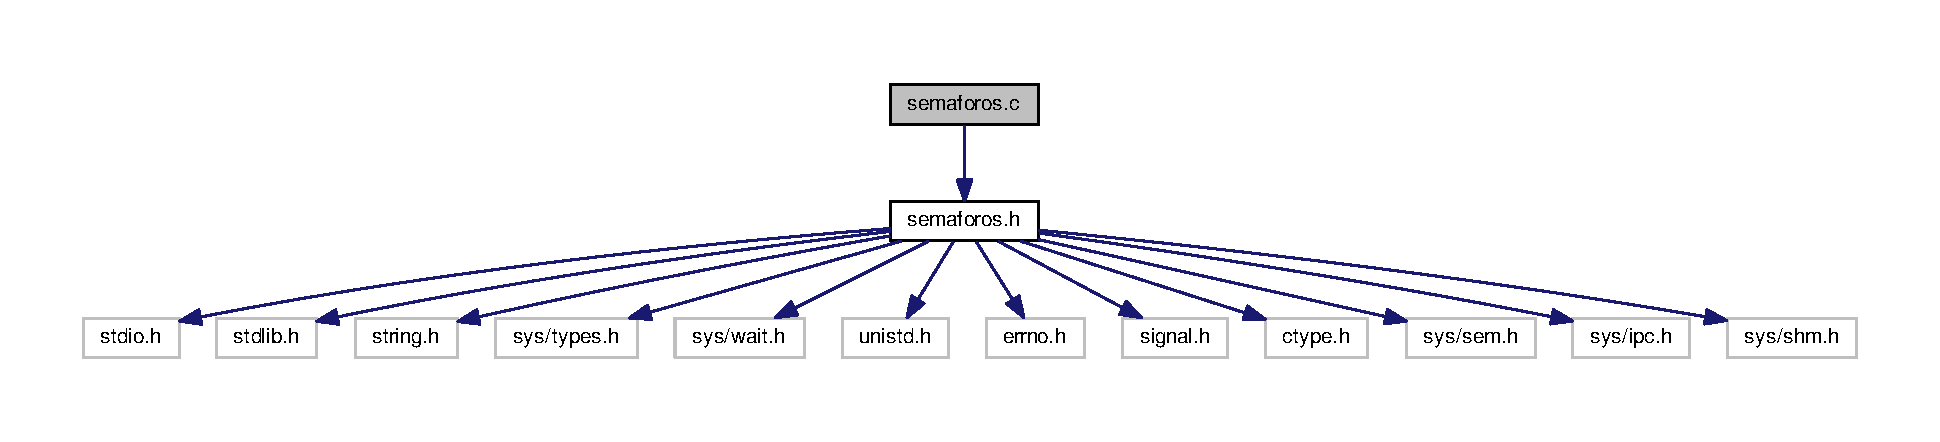
\includegraphics[width=350pt]{semaforos_8c__incl}
\end{center}
\end{figure}
\subsection*{Functions}
\begin{DoxyCompactItemize}
\item 
int \hyperlink{semaforos_8c_a4af104b0ed37e6ae0289a1059bc6e990}{Inicializar\+\_\+\+Semaforo} (int semid, unsigned short $\ast$array)
\begin{DoxyCompactList}\small\item\em funcion inicializadora de semaforos. Su funcionalidad es inicializar los semaforos indicados. \end{DoxyCompactList}\item 
int \hyperlink{semaforos_8c_a731339337960a681efa435a10f12c312}{Borrar\+\_\+\+Semaforo} (int semid)
\begin{DoxyCompactList}\small\item\em funcion que borra semaforos. Su funcionalidad es borrar el semaforo indicado. \end{DoxyCompactList}\item 
int \hyperlink{semaforos_8c_a16b16dd895b5f4cbe48f1ac8977e8b35}{Crear\+\_\+\+Semaforo} (key\+\_\+t key, int size, int $\ast$semid)
\begin{DoxyCompactList}\small\item\em funcion creadora de semaforos. Su funcionalidad es crear un semaforo con la clave y tamaño indicados. \end{DoxyCompactList}\item 
int \hyperlink{semaforos_8c_a883244cd3b83c42cda23687da1b63369}{Down\+\_\+\+Semaforo} (int id, int num\+\_\+sem, int undo)
\begin{DoxyCompactList}\small\item\em funcion que decrementa un semaforo. Su funcionalidad es bajar o decrementar el semaforo indicado. \end{DoxyCompactList}\item 
int \hyperlink{semaforos_8c_ab375ebfc38acbdced46e062a689d5fad}{Down\+Multiple\+\_\+\+Semaforo} (int id, int size, int undo, int $\ast$active)
\begin{DoxyCompactList}\small\item\em funcion que decrementa varios semaforos. Su funcionalidad es bajar o decrementar todos los semaforos indicados. \end{DoxyCompactList}\item 
int \hyperlink{semaforos_8c_a2d5e735aecee4f493898b3d4ebab1a10}{Up\+\_\+\+Semaforo} (int id, int num\+\_\+sem, int undo)
\begin{DoxyCompactList}\small\item\em funcion que incrementa un semaforo. Su funcionalidad es subir o incrementar el semaforo indicado. \end{DoxyCompactList}\item 
int \hyperlink{semaforos_8c_a943759695f018d64a94b8a2c49308092}{Up\+Multiple\+\_\+\+Semaforo} (int id, int size, int undo, int $\ast$active)
\begin{DoxyCompactList}\small\item\em funcion que incrementa varios semaforos. Su funcionalidad es subir o incrementar todos los semaforos indicados. \end{DoxyCompactList}\end{DoxyCompactItemize}


\subsection{Detailed Description}
Ejercicio9. 

Utilidades de manejo de semaforos.

Este ejercicio comprueba la librería de semaforos mientras ayuda didacticamente

\begin{DoxyAuthor}{Author}
Alejandro Santorum \& David Cabornero (G2202-\/\+Pareja7) 
\end{DoxyAuthor}
\begin{DoxyVersion}{Version}
1.\+0 
\end{DoxyVersion}
\begin{DoxyDate}{Date}
06-\/04-\/2018
\end{DoxyDate}
Este modulo contiene la implementacion de las funciones de manejo de semaforos.

\begin{DoxyAuthor}{Author}
Alejandro Santorum \& David Cabornero (G2202-\/\+Pareja7) 
\end{DoxyAuthor}
\begin{DoxyVersion}{Version}
1.\+0 
\end{DoxyVersion}
\begin{DoxyDate}{Date}
01-\/04-\/2018 
\end{DoxyDate}


\subsection{Function Documentation}
\index{semaforos.\+c@{semaforos.\+c}!Borrar\+\_\+\+Semaforo@{Borrar\+\_\+\+Semaforo}}
\index{Borrar\+\_\+\+Semaforo@{Borrar\+\_\+\+Semaforo}!semaforos.\+c@{semaforos.\+c}}
\subsubsection[{\texorpdfstring{Borrar\+\_\+\+Semaforo(int semid)}{Borrar_Semaforo(int semid)}}]{\setlength{\rightskip}{0pt plus 5cm}int Borrar\+\_\+\+Semaforo (
\begin{DoxyParamCaption}
\item[{int}]{semid}
\end{DoxyParamCaption}
)}\hypertarget{semaforos_8c_a731339337960a681efa435a10f12c312}{}\label{semaforos_8c_a731339337960a681efa435a10f12c312}


funcion que borra semaforos. Su funcionalidad es borrar el semaforo indicado. 


\begin{DoxyParams}{Parameters}
{\em semid} & -\/ identificador del semaforo \\
\hline
\end{DoxyParams}
\begin{DoxyReturn}{Returns}
OK si todo fue correcto, E\+R\+R\+OR en caso de error. 
\end{DoxyReturn}
\index{semaforos.\+c@{semaforos.\+c}!Crear\+\_\+\+Semaforo@{Crear\+\_\+\+Semaforo}}
\index{Crear\+\_\+\+Semaforo@{Crear\+\_\+\+Semaforo}!semaforos.\+c@{semaforos.\+c}}
\subsubsection[{\texorpdfstring{Crear\+\_\+\+Semaforo(key\+\_\+t key, int size, int $\ast$semid)}{Crear_Semaforo(key_t key, int size, int *semid)}}]{\setlength{\rightskip}{0pt plus 5cm}int Crear\+\_\+\+Semaforo (
\begin{DoxyParamCaption}
\item[{key\+\_\+t}]{key, }
\item[{int}]{size, }
\item[{int $\ast$}]{semid}
\end{DoxyParamCaption}
)}\hypertarget{semaforos_8c_a16b16dd895b5f4cbe48f1ac8977e8b35}{}\label{semaforos_8c_a16b16dd895b5f4cbe48f1ac8977e8b35}


funcion creadora de semaforos. Su funcionalidad es crear un semaforo con la clave y tamaño indicados. 


\begin{DoxyParams}{Parameters}
{\em key} & -\/ clave precompartida del semaforo \\
\hline
{\em size} & -\/ tamanio del semaforo. \\
\hline
{\em semid} & -\/ entero pasado por referencia para alojar el semid del semaforo creado \\
\hline
\end{DoxyParams}
\begin{DoxyReturn}{Returns}
int $\ast$semid -\/ identificador del semaforo. Int E\+R\+R\+OR en caso de error, 1 si el semaforo ya existia, 0 en caso de exito. 
\end{DoxyReturn}
\index{semaforos.\+c@{semaforos.\+c}!Down\+\_\+\+Semaforo@{Down\+\_\+\+Semaforo}}
\index{Down\+\_\+\+Semaforo@{Down\+\_\+\+Semaforo}!semaforos.\+c@{semaforos.\+c}}
\subsubsection[{\texorpdfstring{Down\+\_\+\+Semaforo(int id, int num\+\_\+sem, int undo)}{Down_Semaforo(int id, int num_sem, int undo)}}]{\setlength{\rightskip}{0pt plus 5cm}int Down\+\_\+\+Semaforo (
\begin{DoxyParamCaption}
\item[{int}]{id, }
\item[{int}]{num\+\_\+sem, }
\item[{int}]{undo}
\end{DoxyParamCaption}
)}\hypertarget{semaforos_8c_a883244cd3b83c42cda23687da1b63369}{}\label{semaforos_8c_a883244cd3b83c42cda23687da1b63369}


funcion que decrementa un semaforo. Su funcionalidad es bajar o decrementar el semaforo indicado. 


\begin{DoxyParams}{Parameters}
{\em id} & -\/ identificador del semaforo \\
\hline
{\em num\+\_\+sem} & -\/ semaforo dentro del array \\
\hline
{\em undo} & -\/ flag de modo persistente pese a finalizacion abrupta \\
\hline
\end{DoxyParams}
\begin{DoxyReturn}{Returns}
OK si todo fue correcto, E\+R\+R\+OR en caso de error. 
\end{DoxyReturn}
\index{semaforos.\+c@{semaforos.\+c}!Down\+Multiple\+\_\+\+Semaforo@{Down\+Multiple\+\_\+\+Semaforo}}
\index{Down\+Multiple\+\_\+\+Semaforo@{Down\+Multiple\+\_\+\+Semaforo}!semaforos.\+c@{semaforos.\+c}}
\subsubsection[{\texorpdfstring{Down\+Multiple\+\_\+\+Semaforo(int id, int size, int undo, int $\ast$active)}{DownMultiple_Semaforo(int id, int size, int undo, int *active)}}]{\setlength{\rightskip}{0pt plus 5cm}int Down\+Multiple\+\_\+\+Semaforo (
\begin{DoxyParamCaption}
\item[{int}]{id, }
\item[{int}]{size, }
\item[{int}]{undo, }
\item[{int $\ast$}]{active}
\end{DoxyParamCaption}
)}\hypertarget{semaforos_8c_ab375ebfc38acbdced46e062a689d5fad}{}\label{semaforos_8c_ab375ebfc38acbdced46e062a689d5fad}


funcion que decrementa varios semaforos. Su funcionalidad es bajar o decrementar todos los semaforos indicados. 


\begin{DoxyParams}{Parameters}
{\em id} & -\/ identificador del semaforo \\
\hline
{\em size} & -\/ tamanio del array de ids de los semaforos involucrados(active) \\
\hline
{\em undo} & -\/ flag de modo persistente pese a finalizacion abrupta \\
\hline
{\em active} & Semaforos involucrados. \\
\hline
\end{DoxyParams}
\begin{DoxyReturn}{Returns}
OK si todo fue correcto, E\+R\+R\+OR en caso de error. 
\end{DoxyReturn}
\index{semaforos.\+c@{semaforos.\+c}!Inicializar\+\_\+\+Semaforo@{Inicializar\+\_\+\+Semaforo}}
\index{Inicializar\+\_\+\+Semaforo@{Inicializar\+\_\+\+Semaforo}!semaforos.\+c@{semaforos.\+c}}
\subsubsection[{\texorpdfstring{Inicializar\+\_\+\+Semaforo(int semid, unsigned short $\ast$array)}{Inicializar_Semaforo(int semid, unsigned short *array)}}]{\setlength{\rightskip}{0pt plus 5cm}int Inicializar\+\_\+\+Semaforo (
\begin{DoxyParamCaption}
\item[{int}]{semid, }
\item[{unsigned short $\ast$}]{array}
\end{DoxyParamCaption}
)}\hypertarget{semaforos_8c_a4af104b0ed37e6ae0289a1059bc6e990}{}\label{semaforos_8c_a4af104b0ed37e6ae0289a1059bc6e990}


funcion inicializadora de semaforos. Su funcionalidad es inicializar los semaforos indicados. 


\begin{DoxyParams}{Parameters}
{\em semid} & -\/ identificador del semaforo \\
\hline
{\em array} & -\/ valores iniciales \\
\hline
\end{DoxyParams}
\begin{DoxyReturn}{Returns}
OK si todo fue correcto, E\+R\+R\+OR en caso de error. 
\end{DoxyReturn}
\index{semaforos.\+c@{semaforos.\+c}!Up\+\_\+\+Semaforo@{Up\+\_\+\+Semaforo}}
\index{Up\+\_\+\+Semaforo@{Up\+\_\+\+Semaforo}!semaforos.\+c@{semaforos.\+c}}
\subsubsection[{\texorpdfstring{Up\+\_\+\+Semaforo(int id, int num\+\_\+sem, int undo)}{Up_Semaforo(int id, int num_sem, int undo)}}]{\setlength{\rightskip}{0pt plus 5cm}int Up\+\_\+\+Semaforo (
\begin{DoxyParamCaption}
\item[{int}]{id, }
\item[{int}]{num\+\_\+sem, }
\item[{int}]{undo}
\end{DoxyParamCaption}
)}\hypertarget{semaforos_8c_a2d5e735aecee4f493898b3d4ebab1a10}{}\label{semaforos_8c_a2d5e735aecee4f493898b3d4ebab1a10}


funcion que incrementa un semaforo. Su funcionalidad es subir o incrementar el semaforo indicado. 


\begin{DoxyParams}{Parameters}
{\em id} & -\/ identificador del semaforo \\
\hline
{\em num\+\_\+sem} & -\/ semaforo dentro del array \\
\hline
{\em undo} & -\/ flag de modo persistente pese a finalizacion abrupta \\
\hline
\end{DoxyParams}
\begin{DoxyReturn}{Returns}
OK si todo fue correcto, E\+R\+R\+OR en caso de error. 
\end{DoxyReturn}
\index{semaforos.\+c@{semaforos.\+c}!Up\+Multiple\+\_\+\+Semaforo@{Up\+Multiple\+\_\+\+Semaforo}}
\index{Up\+Multiple\+\_\+\+Semaforo@{Up\+Multiple\+\_\+\+Semaforo}!semaforos.\+c@{semaforos.\+c}}
\subsubsection[{\texorpdfstring{Up\+Multiple\+\_\+\+Semaforo(int id, int size, int undo, int $\ast$active)}{UpMultiple_Semaforo(int id, int size, int undo, int *active)}}]{\setlength{\rightskip}{0pt plus 5cm}int Up\+Multiple\+\_\+\+Semaforo (
\begin{DoxyParamCaption}
\item[{int}]{id, }
\item[{int}]{size, }
\item[{int}]{undo, }
\item[{int $\ast$}]{active}
\end{DoxyParamCaption}
)}\hypertarget{semaforos_8c_a943759695f018d64a94b8a2c49308092}{}\label{semaforos_8c_a943759695f018d64a94b8a2c49308092}


funcion que incrementa varios semaforos. Su funcionalidad es subir o incrementar todos los semaforos indicados. 


\begin{DoxyParams}{Parameters}
{\em id} & -\/ identificador del semaforo \\
\hline
{\em size} & -\/ tamanio del array de ids de los semaforos involucrados(active) \\
\hline
{\em undo} & -\/ flag de modo persistente pese a finalizacion abrupta \\
\hline
{\em active} & Semaforos involucrados. \\
\hline
\end{DoxyParams}
\begin{DoxyReturn}{Returns}
OK si todo fue correcto, E\+R\+R\+OR en caso de error. 
\end{DoxyReturn}

\hypertarget{semaforos_8h}{}\section{semaforos.\+h File Reference}
\label{semaforos_8h}\index{semaforos.\+h@{semaforos.\+h}}


Utilidades de manejo de semaforos.  


{\ttfamily \#include $<$stdio.\+h$>$}\\*
{\ttfamily \#include $<$stdlib.\+h$>$}\\*
{\ttfamily \#include $<$string.\+h$>$}\\*
{\ttfamily \#include $<$sys/types.\+h$>$}\\*
{\ttfamily \#include $<$sys/wait.\+h$>$}\\*
{\ttfamily \#include $<$unistd.\+h$>$}\\*
{\ttfamily \#include $<$errno.\+h$>$}\\*
{\ttfamily \#include $<$signal.\+h$>$}\\*
{\ttfamily \#include $<$ctype.\+h$>$}\\*
{\ttfamily \#include $<$sys/sem.\+h$>$}\\*
{\ttfamily \#include $<$sys/ipc.\+h$>$}\\*
{\ttfamily \#include $<$sys/shm.\+h$>$}\\*
Include dependency graph for semaforos.\+h\+:
\nopagebreak
\begin{figure}[H]
\begin{center}
\leavevmode
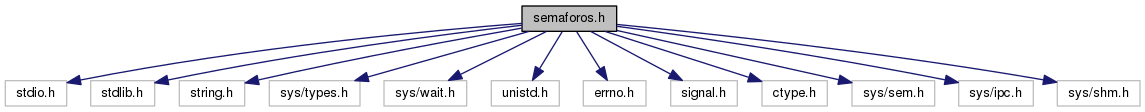
\includegraphics[width=350pt]{semaforos_8h__incl}
\end{center}
\end{figure}
This graph shows which files directly or indirectly include this file\+:
\nopagebreak
\begin{figure}[H]
\begin{center}
\leavevmode
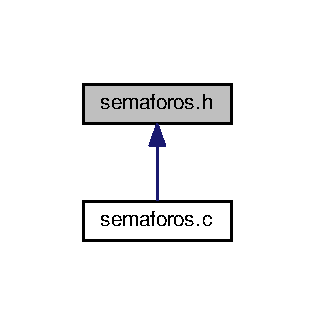
\includegraphics[width=151pt]{semaforos_8h__dep__incl}
\end{center}
\end{figure}
\subsection*{Macros}
\begin{DoxyCompactItemize}
\item 
\#define \hyperlink{semaforos_8h_a8fe83ac76edc595f6b98cd4a4127aed5}{E\+R\+R\+OR}~-\/1
\item 
\#define \hyperlink{semaforos_8h_aba51915c87d64af47fb1cc59348961c9}{OK}~0
\end{DoxyCompactItemize}
\subsection*{Functions}
\begin{DoxyCompactItemize}
\item 
int \hyperlink{semaforos_8h_a4af104b0ed37e6ae0289a1059bc6e990}{Inicializar\+\_\+\+Semaforo} (int semid, unsigned short $\ast$array)
\begin{DoxyCompactList}\small\item\em funcion inicializadora de semaforos. Su funcionalidad es inicializar los semaforos indicados. \end{DoxyCompactList}\item 
int \hyperlink{semaforos_8h_a731339337960a681efa435a10f12c312}{Borrar\+\_\+\+Semaforo} (int semid)
\begin{DoxyCompactList}\small\item\em funcion que borra semaforos. Su funcionalidad es borrar el semaforo indicado. \end{DoxyCompactList}\item 
int \hyperlink{semaforos_8h_a16b16dd895b5f4cbe48f1ac8977e8b35}{Crear\+\_\+\+Semaforo} (key\+\_\+t key, int size, int $\ast$semid)
\begin{DoxyCompactList}\small\item\em funcion creadora de semaforos. Su funcionalidad es crear un semaforo con la clave y tamaño indicados. \end{DoxyCompactList}\item 
int \hyperlink{semaforos_8h_a883244cd3b83c42cda23687da1b63369}{Down\+\_\+\+Semaforo} (int id, int num\+\_\+sem, int undo)
\begin{DoxyCompactList}\small\item\em funcion que decrementa un semaforo. Su funcionalidad es bajar o decrementar el semaforo indicado. \end{DoxyCompactList}\item 
int \hyperlink{semaforos_8h_ab375ebfc38acbdced46e062a689d5fad}{Down\+Multiple\+\_\+\+Semaforo} (int id, int size, int undo, int $\ast$active)
\begin{DoxyCompactList}\small\item\em funcion que decrementa varios semaforos. Su funcionalidad es bajar o decrementar todos los semaforos indicados. \end{DoxyCompactList}\item 
int \hyperlink{semaforos_8h_a2d5e735aecee4f493898b3d4ebab1a10}{Up\+\_\+\+Semaforo} (int id, int num\+\_\+sem, int undo)
\begin{DoxyCompactList}\small\item\em funcion que incrementa un semaforo. Su funcionalidad es subir o incrementar el semaforo indicado. \end{DoxyCompactList}\item 
int \hyperlink{semaforos_8h_a943759695f018d64a94b8a2c49308092}{Up\+Multiple\+\_\+\+Semaforo} (int id, int size, int undo, int $\ast$active)
\begin{DoxyCompactList}\small\item\em funcion que incrementa varios semaforos. Su funcionalidad es subir o incrementar todos los semaforos indicados. \end{DoxyCompactList}\end{DoxyCompactItemize}


\subsection{Detailed Description}
Utilidades de manejo de semaforos. 

Este modulo contiene los prototipos de las funciones de manejo de semaforos.

\begin{DoxyAuthor}{Author}
Alejandro Santorum \& David Cabornero (G2202-\/\+Pareja7) 
\end{DoxyAuthor}
\begin{DoxyVersion}{Version}
1.\+0 
\end{DoxyVersion}
\begin{DoxyDate}{Date}
01-\/04-\/2018 
\end{DoxyDate}


\subsection{Macro Definition Documentation}
\index{semaforos.\+h@{semaforos.\+h}!E\+R\+R\+OR@{E\+R\+R\+OR}}
\index{E\+R\+R\+OR@{E\+R\+R\+OR}!semaforos.\+h@{semaforos.\+h}}
\subsubsection[{\texorpdfstring{E\+R\+R\+OR}{ERROR}}]{\setlength{\rightskip}{0pt plus 5cm}\#define E\+R\+R\+OR~-\/1}\hypertarget{semaforos_8h_a8fe83ac76edc595f6b98cd4a4127aed5}{}\label{semaforos_8h_a8fe83ac76edc595f6b98cd4a4127aed5}
Constante con significado de operacion erronea \index{semaforos.\+h@{semaforos.\+h}!OK@{OK}}
\index{OK@{OK}!semaforos.\+h@{semaforos.\+h}}
\subsubsection[{\texorpdfstring{OK}{OK}}]{\setlength{\rightskip}{0pt plus 5cm}\#define OK~0}\hypertarget{semaforos_8h_aba51915c87d64af47fb1cc59348961c9}{}\label{semaforos_8h_aba51915c87d64af47fb1cc59348961c9}
Constante con significado de operacion exitosa 

\subsection{Function Documentation}
\index{semaforos.\+h@{semaforos.\+h}!Borrar\+\_\+\+Semaforo@{Borrar\+\_\+\+Semaforo}}
\index{Borrar\+\_\+\+Semaforo@{Borrar\+\_\+\+Semaforo}!semaforos.\+h@{semaforos.\+h}}
\subsubsection[{\texorpdfstring{Borrar\+\_\+\+Semaforo(int semid)}{Borrar_Semaforo(int semid)}}]{\setlength{\rightskip}{0pt plus 5cm}int Borrar\+\_\+\+Semaforo (
\begin{DoxyParamCaption}
\item[{int}]{semid}
\end{DoxyParamCaption}
)}\hypertarget{semaforos_8h_a731339337960a681efa435a10f12c312}{}\label{semaforos_8h_a731339337960a681efa435a10f12c312}


funcion que borra semaforos. Su funcionalidad es borrar el semaforo indicado. 


\begin{DoxyParams}{Parameters}
{\em semid} & -\/ identificador del semaforo \\
\hline
\end{DoxyParams}
\begin{DoxyReturn}{Returns}
OK si todo fue correcto, E\+R\+R\+OR en caso de error. 
\end{DoxyReturn}
\index{semaforos.\+h@{semaforos.\+h}!Crear\+\_\+\+Semaforo@{Crear\+\_\+\+Semaforo}}
\index{Crear\+\_\+\+Semaforo@{Crear\+\_\+\+Semaforo}!semaforos.\+h@{semaforos.\+h}}
\subsubsection[{\texorpdfstring{Crear\+\_\+\+Semaforo(key\+\_\+t key, int size, int $\ast$semid)}{Crear_Semaforo(key_t key, int size, int *semid)}}]{\setlength{\rightskip}{0pt plus 5cm}int Crear\+\_\+\+Semaforo (
\begin{DoxyParamCaption}
\item[{key\+\_\+t}]{key, }
\item[{int}]{size, }
\item[{int $\ast$}]{semid}
\end{DoxyParamCaption}
)}\hypertarget{semaforos_8h_a16b16dd895b5f4cbe48f1ac8977e8b35}{}\label{semaforos_8h_a16b16dd895b5f4cbe48f1ac8977e8b35}


funcion creadora de semaforos. Su funcionalidad es crear un semaforo con la clave y tamaño indicados. 


\begin{DoxyParams}{Parameters}
{\em key} & -\/ clave precompartida del semaforo \\
\hline
{\em size} & -\/ tamanio del semaforo. \\
\hline
{\em semid} & -\/ entero pasado por referencia para alojar el semid del semaforo creado \\
\hline
\end{DoxyParams}
\begin{DoxyReturn}{Returns}
int $\ast$semid -\/ identificador del semaforo. Int E\+R\+R\+OR en caso de error, 1 si el semaforo ya existia, 0 en caso de exito. 
\end{DoxyReturn}
\index{semaforos.\+h@{semaforos.\+h}!Down\+\_\+\+Semaforo@{Down\+\_\+\+Semaforo}}
\index{Down\+\_\+\+Semaforo@{Down\+\_\+\+Semaforo}!semaforos.\+h@{semaforos.\+h}}
\subsubsection[{\texorpdfstring{Down\+\_\+\+Semaforo(int id, int num\+\_\+sem, int undo)}{Down_Semaforo(int id, int num_sem, int undo)}}]{\setlength{\rightskip}{0pt plus 5cm}int Down\+\_\+\+Semaforo (
\begin{DoxyParamCaption}
\item[{int}]{id, }
\item[{int}]{num\+\_\+sem, }
\item[{int}]{undo}
\end{DoxyParamCaption}
)}\hypertarget{semaforos_8h_a883244cd3b83c42cda23687da1b63369}{}\label{semaforos_8h_a883244cd3b83c42cda23687da1b63369}


funcion que decrementa un semaforo. Su funcionalidad es bajar o decrementar el semaforo indicado. 


\begin{DoxyParams}{Parameters}
{\em id} & -\/ identificador del semaforo \\
\hline
{\em num\+\_\+sem} & -\/ semaforo dentro del array \\
\hline
{\em undo} & -\/ flag de modo persistente pese a finalizacion abrupta \\
\hline
\end{DoxyParams}
\begin{DoxyReturn}{Returns}
OK si todo fue correcto, E\+R\+R\+OR en caso de error. 
\end{DoxyReturn}
\index{semaforos.\+h@{semaforos.\+h}!Down\+Multiple\+\_\+\+Semaforo@{Down\+Multiple\+\_\+\+Semaforo}}
\index{Down\+Multiple\+\_\+\+Semaforo@{Down\+Multiple\+\_\+\+Semaforo}!semaforos.\+h@{semaforos.\+h}}
\subsubsection[{\texorpdfstring{Down\+Multiple\+\_\+\+Semaforo(int id, int size, int undo, int $\ast$active)}{DownMultiple_Semaforo(int id, int size, int undo, int *active)}}]{\setlength{\rightskip}{0pt plus 5cm}int Down\+Multiple\+\_\+\+Semaforo (
\begin{DoxyParamCaption}
\item[{int}]{id, }
\item[{int}]{size, }
\item[{int}]{undo, }
\item[{int $\ast$}]{active}
\end{DoxyParamCaption}
)}\hypertarget{semaforos_8h_ab375ebfc38acbdced46e062a689d5fad}{}\label{semaforos_8h_ab375ebfc38acbdced46e062a689d5fad}


funcion que decrementa varios semaforos. Su funcionalidad es bajar o decrementar todos los semaforos indicados. 


\begin{DoxyParams}{Parameters}
{\em id} & -\/ identificador del semaforo \\
\hline
{\em size} & -\/ tamanio del array de ids de los semaforos involucrados(active) \\
\hline
{\em undo} & -\/ flag de modo persistente pese a finalizacion abrupta \\
\hline
{\em active} & Semaforos involucrados. \\
\hline
\end{DoxyParams}
\begin{DoxyReturn}{Returns}
OK si todo fue correcto, E\+R\+R\+OR en caso de error. 
\end{DoxyReturn}
\index{semaforos.\+h@{semaforos.\+h}!Inicializar\+\_\+\+Semaforo@{Inicializar\+\_\+\+Semaforo}}
\index{Inicializar\+\_\+\+Semaforo@{Inicializar\+\_\+\+Semaforo}!semaforos.\+h@{semaforos.\+h}}
\subsubsection[{\texorpdfstring{Inicializar\+\_\+\+Semaforo(int semid, unsigned short $\ast$array)}{Inicializar_Semaforo(int semid, unsigned short *array)}}]{\setlength{\rightskip}{0pt plus 5cm}int Inicializar\+\_\+\+Semaforo (
\begin{DoxyParamCaption}
\item[{int}]{semid, }
\item[{unsigned short $\ast$}]{array}
\end{DoxyParamCaption}
)}\hypertarget{semaforos_8h_a4af104b0ed37e6ae0289a1059bc6e990}{}\label{semaforos_8h_a4af104b0ed37e6ae0289a1059bc6e990}


funcion inicializadora de semaforos. Su funcionalidad es inicializar los semaforos indicados. 


\begin{DoxyParams}{Parameters}
{\em semid} & -\/ identificador del semaforo \\
\hline
{\em array} & -\/ valores iniciales \\
\hline
\end{DoxyParams}
\begin{DoxyReturn}{Returns}
OK si todo fue correcto, E\+R\+R\+OR en caso de error. 
\end{DoxyReturn}
\index{semaforos.\+h@{semaforos.\+h}!Up\+\_\+\+Semaforo@{Up\+\_\+\+Semaforo}}
\index{Up\+\_\+\+Semaforo@{Up\+\_\+\+Semaforo}!semaforos.\+h@{semaforos.\+h}}
\subsubsection[{\texorpdfstring{Up\+\_\+\+Semaforo(int id, int num\+\_\+sem, int undo)}{Up_Semaforo(int id, int num_sem, int undo)}}]{\setlength{\rightskip}{0pt plus 5cm}int Up\+\_\+\+Semaforo (
\begin{DoxyParamCaption}
\item[{int}]{id, }
\item[{int}]{num\+\_\+sem, }
\item[{int}]{undo}
\end{DoxyParamCaption}
)}\hypertarget{semaforos_8h_a2d5e735aecee4f493898b3d4ebab1a10}{}\label{semaforos_8h_a2d5e735aecee4f493898b3d4ebab1a10}


funcion que incrementa un semaforo. Su funcionalidad es subir o incrementar el semaforo indicado. 


\begin{DoxyParams}{Parameters}
{\em id} & -\/ identificador del semaforo \\
\hline
{\em num\+\_\+sem} & -\/ semaforo dentro del array \\
\hline
{\em undo} & -\/ flag de modo persistente pese a finalizacion abrupta \\
\hline
\end{DoxyParams}
\begin{DoxyReturn}{Returns}
OK si todo fue correcto, E\+R\+R\+OR en caso de error. 
\end{DoxyReturn}
\index{semaforos.\+h@{semaforos.\+h}!Up\+Multiple\+\_\+\+Semaforo@{Up\+Multiple\+\_\+\+Semaforo}}
\index{Up\+Multiple\+\_\+\+Semaforo@{Up\+Multiple\+\_\+\+Semaforo}!semaforos.\+h@{semaforos.\+h}}
\subsubsection[{\texorpdfstring{Up\+Multiple\+\_\+\+Semaforo(int id, int size, int undo, int $\ast$active)}{UpMultiple_Semaforo(int id, int size, int undo, int *active)}}]{\setlength{\rightskip}{0pt plus 5cm}int Up\+Multiple\+\_\+\+Semaforo (
\begin{DoxyParamCaption}
\item[{int}]{id, }
\item[{int}]{size, }
\item[{int}]{undo, }
\item[{int $\ast$}]{active}
\end{DoxyParamCaption}
)}\hypertarget{semaforos_8h_a943759695f018d64a94b8a2c49308092}{}\label{semaforos_8h_a943759695f018d64a94b8a2c49308092}


funcion que incrementa varios semaforos. Su funcionalidad es subir o incrementar todos los semaforos indicados. 


\begin{DoxyParams}{Parameters}
{\em id} & -\/ identificador del semaforo \\
\hline
{\em size} & -\/ tamanio del array de ids de los semaforos involucrados(active) \\
\hline
{\em undo} & -\/ flag de modo persistente pese a finalizacion abrupta \\
\hline
{\em active} & Semaforos involucrados. \\
\hline
\end{DoxyParams}
\begin{DoxyReturn}{Returns}
OK si todo fue correcto, E\+R\+R\+OR en caso de error. 
\end{DoxyReturn}

%--- End generated contents ---

% Index
\backmatter
\newpage
\phantomsection
\clearemptydoublepage
\addcontentsline{toc}{chapter}{Index}
\printindex

\end{document}
